\documentclass{article}
\usepackage[utf8]{inputenc}
\usepackage{CJKutf8}

\title{Immune algorithm report}

\author{\begin{CJK*}{UTF8}{gbsn}
谌正/21721122\end{CJK*} }





\date{April 2018}

\usepackage{natbib}
\usepackage{graphicx}

\begin{document}

\maketitle


\section{Introduction}
Artificial Immune Systems(AISs) represent a field of theories,principles,and concepte of modern immunology to design immune system-based applications in science and engineering \citep{a14}.One role of the immune system is to protect the host organism against attacks from antigens and eliminate those cells that have been "infected".AISs are proving to be a very general and applicable form of bio-inspired computing.Agreat deal of work has gone into developing algorithms that extrapolate basic immune processes such as clonal selection,negative and positive selection,danger theory,and immune net works\citep{a2}.To date,AIShave been applied to areas such as machine learning\citep{a3},optimization\citep{a4},bioinformatics\citep{a5},robotic systems\citep{a6},decision support systems\citep{a7},network intrusion detection\citep{a8},combinatorial optimization\citep{a9},scheduling\citep{a10},anomaly detection\citep{a11},fault diagnosis\citep{a12},computer security[\citep{a13},data analysis\citep{a1},and many other areas.
This report is structured as follows: 
\newline
$1$.introduces a classic immune algorithm 
\newline
$2$. for the problems existing in the classical immune algorithm, and improves it 
\newline
$3$. for the combinatorial optimization problem: TSP problem, and proposes an immune model.


\section{Immune Algorithm}
\begin{figure}
\centering
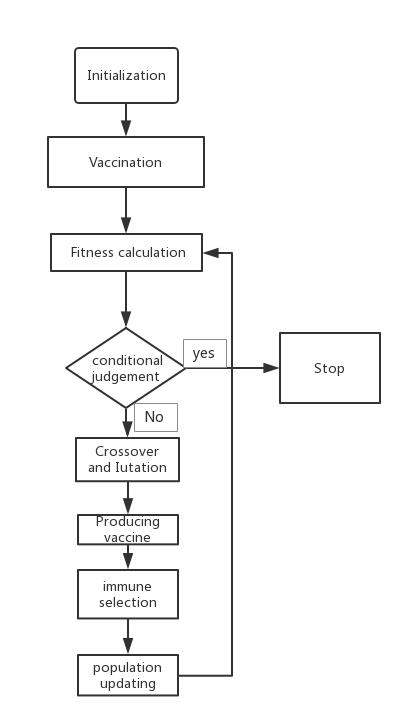
\includegraphics[scale=0.4]{immune.png}
\end{figure}
\subsection{Immune Operator}
\indent

 \par\setlength\parindent{1em}
   1.Full immunity refers to the type of immunity that each group of individuals in a group has an immune operation on every link after the action of genetic operators. It is mainly applied to the initial stage of individual evolution, but not in the process of evolution.
   \par\setlength\parindent{1em}
   2.The target immunity refers to a type of immune response at the point of action only after a genetic operation.The target immunization is generally associated with the whole process of population evolution,and it is a basic operator of the immune operation.
  
\subsection{The actual operation process of immune algorithm}
\indent

 \par\setlength\parindent{1em}
 1.The specific analysis of the solved problems(regarded as an antigen)
 \par\setlength\parindent{1em}
 2.This feature information is processed to transform it into a solution to the problem(The set of solutions obtained according to the scheme is called the antibody based on the vaccine abov)
\par\setlength\parindent{1em}
 3.Transform this scheme into an immune operator in an appropriate form
 \subsection{Vaccination}
 According to the prior knowledge, some genes in $X$ are modified to make the individual have higher fitness for greater probability. 
 \subsection{Immune selection}
\indent

 \par\setlength\parindent{1em}
(1)Immunoassay:The detection of individuals vaccinated is not as good as the parent, indicating that the phenomenon of severe degeneration has occurred during the process of crossover and mutation, and this individual will be replaced by the corresponding individuals in the parent.
\par\setlength\parindent{1em}
(2)Annealing selection:
In the current progeny group $E_k=(x_1,...,x_{n_0})$, 

the individual Xi is selected by the probability $P(x_i)$ to enter the new parent group:
\par\setlength\parindent{6em}
$P(x_i)=e^{f(x_i)/T_k}\sum_{i=1}^{n_0}e^{f(xi)/T_k}$
\par\setlength\parindent{6em}
$f(x_i)$ is the adaptive degree of individual,
\par\setlength\parindent{6em}
$T_k$is a temperature control sequence approaching 0.



\section{Immune Operator}
\subsection{The execution algorithm of immune operator}
$a_{H,k}^i$ is the antibody obtained after vaccinating the k generation the i individual $a_k^i$. $P_I$ is the probability of vaccinating individuals, and $P_V$ is the probability of updating the vaccine. $V(a_k^i,h_j)$ is an inoculation operation modifing the gene on an individual$a_k^i$ according to the pattern $h_j$,  and N and m are the size of the population and the vaccine, respectively.$f(x)$represent the fitness of individual x.



\par\setlength\parindent{6em}
Begin:
\par\setlength\parindent{6em}
Extraction of vaccine:
  \par\setlength\parindent{8em}
  Analyze the problem to be asked and collect the characteristic information
  \par\setlength\parindent{8em}
  Estimation of patterns on specific gene sites based on characteristic information:$H={h_j|j=1,2,...,m}$
   \par\setlength\parindent{6em}
   $k=0$and$j=0$;
   \par\setlength\parindent{6em}
   while(Conditions=true)
   \par\setlength\parindent{7em}
    if{$P_v$}=true,then $j=j+1$;
    \par\setlength\parindent{7em}
    $i=0$;
    \par\setlength\parindent{7em}
    for($i<=n$)
    \par\setlength\parindent{8em}
    Vaccination:$a_{H,k}^j=V_{p_I}{(a_k^i,h_j)}$;
    \par\setlength\parindent{8em}
    Immunoassay:if $f(a_{H,k}^i)<f(a_{k-1}^i)$,then $a_k^j=a_{k-1}^i$;
    else $a_k^i=a_{H,k}^i$;
    \par\setlength\parindent{8em}
    $i=i+1$;
    \par\setlength\parindent{7em}
    Annealing selection:$A_{k+1}=S(A_k)$;
    \par\setlength\parindent{7em}
    $k=k+1$;
    
    End



\section{Improved Immune Algorithm}
In the traditional artificial immune optimization algorithm, for cloning operator, the number of antibodies is preset, not determined by affinity. The mutation operator in the traditional artificial immune optimization algorithm is to conducting Gauss mutation at random.
The improved immune optimization algorithm proposed in this paper improves the cloning and mutation steps of the traditional artificial immune algorithm, in which the clone number is proportional to the affinity of the parent antibody, and the mutation level of each antibody is inversely proportional to the affinity of the parent antibody in the mutation. At the same time, in the improved immune optimization algorithm, the excellent learning mechanism of the antibody is added, that is, the mutation process of each antibody will not only inherit the advantages of the parent antibody, but also learn from the antibody with the most affinity in the current population antibody.
Therefore, the complete antibody clone equation can be described as follows:
  \par\setlength\parindent{7em}
$h_i(t)=norm(Aff(Ab_i(t)))$
\newline
  \par\setlength\parindent{7em}
  \par\setlength\parindent{7em}
$C_i(t+1)=r_1C_{max}H^n(t)+C_0$
\par\setlength\parindent{1em}
Among them, $t$represents the number of iterations. $norm()$is a normalized function.$h_i(t)$is the value of the normalized function,$Aff()$is an affinity function of antibodies, $C_{max}$ is the largest clone of antibodies,$r_1$ is a random number in [0, 1],$n$ is the exponent of power function, $C_0$is the clone base of antibodies, $C_i(t+1)$ is the clone number of antibody$Ab_i(t)$, and $H^n(t)$ is antibody clone factor.when $n=1$, the number of antibody clones is proportional to affinity. When $n> 1$, the greater the affinity, the faster the number of clones grows. When $n<1$the number of antibody clones with small affinity was larger. However,in the improved immune algorithm, choosng the appropriate power exponent n is very important for the size of antibody population and complexity of the algorithm. The relationship between the number of antibody clones and affinity of antibody is influenced by antibody clone factor.
\par\setlength\parindent{1em}
In Gauss mutation, we use affinity based Gauss function to adjust the level of antibody variation. The antibody variation equation of the algorithm is as follows:
\par\setlength\parindent{7em}
$\Delta Ab_i(t+1)=\beta\gamma
exp(-h_i(t)/\eta)$
\par\setlength\parindent{1em}
Among them, the $\eta$ is the control factor, the $\gamma$ is the multiple of variation, the $\beta$ is the random number in [0, 1], and the
$\Delta Ab_i(t+1)$is the variation value between the parent antibody and the sub antibody, and the rest of the variables are the same as the equation (1).If $\eta$ is  greater, variation is higher; and vice versa. The control factor $\eta$ has a big effect on efficiency of the evolution of the immune algorithm.
\par\setlength\parindent{1em}
After learning, an evolved sub antibody not only carries the variation information from the parent antibody, but also focuses on learning the best antibodies in the group:
\par\setlength\parindent{7em}
$\Delta Ab_i^*(t+1)= \omega^*(Ab_g(t)-Ab(t))$
\newline
$\omega $ is the random number in [0, 1]. $ Ab_g(t)$ is the global best antibody. $\Delta Ab_i^*(t+1)$is the learning information of$t + 1$ generation. Weight coefficients $k_1$ and $k_2$ are used to balance the contribution of $\Delta Ab_i(t+1)$ and $\Delta Ab_i^*(t+1)$ to antibody evolution, respectively. In mutation operation, we need to skillfully treat excellent antibodies and non excellent antibodies. For excellent antibodies, excellent retention and affinity learning strategies are carried out according to affinity; and for non excellent antibodies, excellent learning strategies are also carried out in addition to excellent retention and affinity learning strategies. Therefore, the evolution of antibodies can be carried out according to the following formula.
\newline 
When $Ab_g(t)=Ab_i(t)$
\par\setlength\parindent{7em}
$Ab_i(t+1)=Ab_i(t)+ \Delta Ab_i(t+1)$
\newline 
When$Ab_g(t)\neq Ab_i(t)$
\par\setlength\parindent{7em}
$Ab_i(t+1)=Ab_i(t)+k_1\Delta Ab_i(t+1)+k_2\Delta Ab_i^*(t+1)$
\par\setlength\parindent{1em}
From the formula above, we know that the new candidate antibodies are composed of three items: the first is the parent antibody information, the second is the affinity learning information, and the third is the excellent learning information. In order to speed up the search speed of the algorithm, it is necessary to make a balance between increasing $k_1$and reduce$k_2$
\section{
Immune algorithm model for TSP problem}
\subsection{Analyze the problem to be solved and collect the characteristic information}


 Suppose a person starts from a city at a certain time and wants to go to the next target city. Generally, the first choice is the nearest city to the local route. If the target city is just a city ahead of the city, then,it will be replaced by the city with the smallest distance other than this city.This method is not a solution to the global problem, but in a very small range, such as the only three or four cities (relative to the global problem, which belongs to a local problem), this consideration is often a better strategy. Of course, whether it can be the final solution still
need futher judgment.
\subsection{Making immune vaccines based on characteristic information}
Based on the above understanding, in terms of the characteristics of the TSP problem, in the final solution,that is the selection of the best path, including and in a large degree, includes the shortest distance between adjacent cities. This characteristic of the TSP problem can be used as a characteristic information or knowledge for the solution of the problem, so that it can be viewed as a reference. In order to extract the vaccine from the problem, in the specific implementation process, it is only necessary to use a general cyclic iterative method to find out the neighboring cities of all cities (of course, a city may be a neighboring city of two or more cities, and probably not. "
The vaccine is not an individual, so it can not be used as a solution to the problem . It only has the characteristics of individuals in some gene locations.
\subsection{Vaccination}
\begin{figure}[h!]
\centering
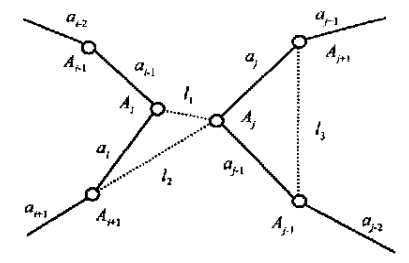
\includegraphics[scale=0.8]{path}
\end{figure}


Generally,suppose that,in the TSP problem, all cities nearest to $A_i$ are $A_j$,and the two part is not directly connected, but is in the two segment of a certain path
\par\setlength\parindent{7em}
$A_{i-1}-A_i-A_{i+1}$and$A_{j-1}-A_j-A_{j+1}$.
\newline
As shown in the figure above,The current traversal path is
\par\setlength\parindent{7em}
$\pi={A_0,...,A_{i-1},A_i,A_{i+1},...,A_{j-1},A_j,A_{j+1},...,A_N}$
\newline
its corresponding path length is:
\par\setlength\parindent{7em}
$D_{\pi}=\sum_{k=1}^{i-1}a_k+a_i+\sum_{k=i+1}^{i-2}a_k+a_{j-1}+a_j+\sum_{k=j+1}^{N}a_k $.
\newline
Under the condition of the immune probability $P_i$, for the city$A_i$, the immune operator will arrange its adjacent city$A_j$into his next target city, then the original traversal path is adjusted as follow:
\par\setlength\parindent{7em}
$\pi={A_0,...,A_{i-1},A_i,A_j,A_{i+1},...,A_{j-1},A_{j+1},...,A_N}$
\newline
then the length of the path is adjusted as follows
\par\setlength\parindent{7em}
$D_{\pi_c}=\sum_{k=1}^{i-1}a_k+l_1+l_2+\sum_{k=i+1}^{i-2}a_k+l_3 +\sum_{k=j+1}^{N}a_k $
\newline
Because$A_j$is the nearest point from $A_i$ in all cities,$l_1$ must be the shortest or the sub short side in the triangle made up of $A_i-A_j-A_{i+1}$ (at this time $l_2$ must be the shortest side.for the reason that if $a_i<l_1$,then the most nearst city from $A_i$will be $A_{i+1}$rather than $A_j$);However,between $A_{j-1},A_j,A_{j+1}$,this property does not necessarily exists, so in most cases, the reduction of $l_3$ to $a_{j-1}+a_j$  is greater than the increasement of $l_1+l_2$ to $a_i$.
In this local environment, the operator makes a best adjustment to the path. Of course,whether this adjustment can contribute to the whole path still needs futher study.  However,it is not difficult to make the following relationship from the analysis process:
\par\setlength\parindent{7em}
$P(D_{\pi_c}<D_{\pi})>>P(D_{\pi_c}>D_{\pi})$
\
\newline
The so-called "adjustment" process is immune injection process based on a specific vaccine when solving the TSP problem.

\bibliographystyle{plain}
\bibliography{references}


\end{document}
